\documentclass{article}
\usepackage[T2A]{fontenc}
\usepackage{empheq}

\hyphenation{ма-те-ма-ти-ка вос-ста-нав-ли-вать}
\usepackage[english, russian]{babel}
\usepackage{amsmath}
\usepackage{graphicx}
\usepackage{amssymb}
\graphicspath{ {./images/} }
\begin{document}
 
\tableofcontents

\section{Натуральные числа}

\begin{itemize}
\item[] В зависимости от области математики в множество натуральных чисел может включаться ноль:
  \begin{itemize}
  \item В теории чисел: $1, 2, 3, \ldots$
  \item В математической логике: $0, 1, 2, 3, \ldots$
  \end{itemize}

\item[] В аппаратуре для представления натуральных чисел используют двоичную запись числа 
(были также машины с десятичной и троичной системой, например машина "Сетунь"). 
Для представления числа отводится 32 бита или 64 бита. Из-за этого ограничения мы не можем представить все натуральные числа.

\item[] В языках программирования используются беззнаковые числа с диапазоном $0 \ldots 2^{64}-1$. 
Представлены не все числа, а только до определённого предела.

\item[] В системах символьных вычислений обычно нет явного предела, он определяется размером оперативной памяти компьютера.
\end{itemize}

\section{Ноль}
\paragraph{}

\begin{itemize}
\item[] В математике +0 = -0, в тоже время в аппаратуре это не так, аппаратно может быть два нуля, +0 и -0. Это приводит к тому, что
если надо проверить x >= y то нужно выполнить операцию x - y и посмотреть на знаковый бит разности, если знаковый бит положительный, то считаем,
что x больше или равен y, а если отрицателен, то нет. Откуда знаковый бит разности:
\[
x - x = \begin{cases}
+0 & \text{, если } $x >= 0$ \\
-0 & \text{, если} $x < 0$
\end{cases}
\]
\[
x >= x = \begin{cases}
true & \text{, если } $x >= 0$ \\
false & \text{, если} $x < 0$
\end{cases}
\]
Подобный подход с 2 нулями существует и сегодня.
\item[] В некоторых языках программирования также предусмотрены 2 нуля, например в языке Julia, 
но если задать выражение 0.0 == -0.0, программа даст true. Также при сравнении чисел на комплексной плоскости $-1+0.0i == -1-0.0i$ программа выдаёт true.
Ещё один эксперемент будет ли sqrt($-1+0.0i$) == sqrt($-1-0.0i$) программа выдаст false, т.к. sqrt($-1+0.0i$) = $0.0+1.0i$ а sqrt($-1-0.0i$) = $0.0-1.0i$
ради такой возможности в частности и допускаются 2 нуля, чтобы различить корень квадратный из минус единицы.
\item[] В символьным вычислениях, могут получаться досточно не ожиданные результаты. Например, есть у нас интеграл


Вычисление в Mathematica:
\[
\texttt{Integrate[x\^{}(a-1) /. a->0, x]} \quad \text{даёт} \quad \log x
\]

\[
\left. \int x^{a-1} \, dx \right|_{a=0} = \int \frac{dx}{x} = \ln|x| + C
\]

Вычисление в Mathematica:
\[
\texttt{Integrate[x\^{}(a-1), x] /. a->0} \quad \text{даёт} \quad \texttt{Indeterminate}
\]
Наша программа не задумывается, что наше значение может быть равно 0 и мы подставили значение на котором система ломается.


Математически корректный подход:
\[
\int x^{a-1} dx = 
\begin{cases}
\frac{x^a}{a} + C & \text{при } a \neq 0 \\
\ln|x| + C & \text{при } a = 0
\end{cases}
\]

\end{itemize}

\section{Целые числа}
\paragraph{}

\begin{itemize}
\item[] В аппаратуре под них отводится также ограниченное количество битов, но в отличии от натуральных, тут 1 бит отводится под знак.
Например в языке julia тип данных int32: имеет диапазон $-2^{31}$...$2^{31}-1$. Также в языках, есть неявное приведение типов, то есть x=$2^{31}-1$ (2147483647)
и введем команду x+1 то получим число 2147483648 т.к. он приведён к int64: диапазон $-2^{63}$...$2^{63}-1$
\end{itemize}   

\section{Рациональные числа}
\paragraph{}
\begin{itemize}
\item[] Аппаратной реализации рациональных чисел нет.
\item[] Язык программирования воспринимает рациональные числа просто как упорядоченные пары целых чисел и допускают такое число 
которое можно интерпретировать как плюс бесконечность. Например, в языке julia 5//0 получим 1//0 или -5//0 получим -1//0.
\end{itemize}   

\section{Алгебраические числа}
\paragraph{}

\begin{itemize}
\item[] Пример алгебраического числа это $\sqrt{2}$ или выражение из радикалов. Формально алгебраическое число - это корень
уравнения вида \[ a_nx^n + a_{n-1}x^{n-1} + \cdots + a_1x + a_0 = 0 \] где $[a_0, a_1, \dots, a_{n-1}, a_n]$ — целые числа.

Вещественное алгебраическое число можно задать, указав уравнение описанное выше и два рациональных числа b и c такие, что существует ровно одно 
значение удовлетворяющее уравнению выше и неравенствам b < x < c.
\item[] Аппаратная реализация, как правило очень слабая. Например существует аппаратная реализация извлечения квадратного корня.
\end{itemize}   


\section{Вещественные числа}
\paragraph{}

\begin{itemize}
\item[] Вещественные числа это двоичные или бесконечные числа, но имеющие неограниченную мантиссу. 
В программирование есть типы данных real или float, что соответствует типу вещественное число. Реально вычисления производятся
с конечным множеством двоично-рациональных чисел вида $\frac{m}{2^n}$. Арифметические операции над такими числами выполняются
приближённо. Данный проблема приводит к тому что a + b = b + a - обычно выполняется, a + (b + c) = (a + b) + c может не выполнятся.


\textbf{Интервальная арифметики}


\item[] Интервал [a, b] представляет множество \{x | a <= x <= b\}. Функцию y=f(x) можно расширить на интервалы:
f([a,b]) = [c,d] = [inf f(x), sup f(x)]

Основное свойство:
\[ a \leq x \leq b \implies c \leq f(x) = y \leq d \]
\item[] Явные формулы для арифметических операций:
\item[]Сложение
\[ [a_1, b_1] + [a_2, b_2] = [a_1 + b_2, b_1 + a_2] \]
\[ a_1 \leq x_1 \leq b_1 \& a_2 \leq x_2 \leq b_2 \implies a_1 + a_2 \leq x_1 + x_2 \leq b_1 + b_2 \]
\item[] Вычитание
\[ [a_1, b_1] - [a_2, b_2] = [a_1 - b_2, b_1 - a_2] \]
\[ a_1 \leq x_1 \leq b_1 \& a_2 \leq x_2 \leq b_2 \implies a_1 - a_2 \leq x_1 - x_2 \leq b_1 - b_2 \]
\item[] Умножение
 $[a_1, b_1] \times [a_2, b_2] = $
$= \bigl[\min(a_1 b_1, a_1 b_2, a_2 b_1, a_2 b_2),\ \max(a_1 b_1, a_1 b_2, a_2 b_1, a_2 b_2)\bigr]$
\item[] Интервальная арифметика не получила широкого распространения. Допустить у нас есть правила действий и если наши границы 
это произвольные рациональные числа, то будет всё хорошо, но при этом будут быстро расти числители и знаменатели, каждое действие
может удваивать знаменатель.
\item[] Чтобы избежать этого можно сказать, что концы интервала будут машинными числами. Нужно использовать направленное округление:
\[ [a_1, b_1] + [a_2, b_2] = [a_1 + {\downarrow} a_2, b_1 + {\uparrow} b_2] \]
Cложение с округлением вниз:
\[ x +{\downarrow} y \leq x + y \]
Cложение с округлением вверх:
\[ x + y \leq x +{\uparrow} y \]
Складывая интервалы с машинными числами можно получить интервал с машинными числами, который заведомо содержит истинное 
значение суммы этот интервал будет чуть шире, чем минимально возможный, но его машинная точность будет умещаться в обычных числах.
Свойство:
\[ a_1 \leq x_1 \leq \& a_2 \leq x_2 \leq b_2 \implies a_1 +{\downarrow} a_2 \leq x_1 + x_2 \leq b_1 +{\uparrow} b_2\]
\item[] Интервальные вычисления реализованы в системы Arb  используется в python-flint и sage.
\item[] Существует стандарт ISO 60559:2020. В нем сказано, что для каждой из четырёх математических операций
(сложение, вычитание, умножение, деление) в аппаратуре должно быть 5 вариантов. Эти варианты отличаются округлением. Когда 
мы можем управлять округлением в меньшую и большую сторону, то реализация интервальной арифметики становится более простой.
\end{itemize} 
\section{Комплексные числа}
\paragraph{}

\begin{itemize}
\item[] [a, b + i[c,d]] представляет множество \[\{z| a \leq Re(z) \leq b \& c \leq Im(z) \leq d \}\]
Интервальная арифметика
\[([1,4] + i[1,2]) \times ([1,1] + i[1,1]) = \text{?}\]
\[\{z_1 \times z_2 | z_1 \in [1,4] + i[1,2] \& z_2 \in [1,1] + i[1,1]\}\]
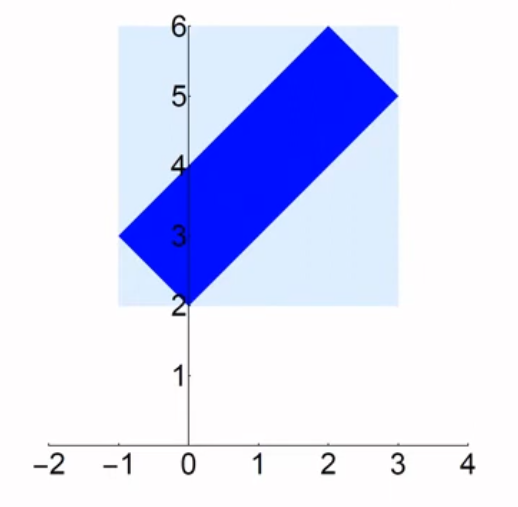
\includegraphics[width=0.8\textwidth, keepaspectratio]{./images/compl.png}
\[([1,4] + i[1,2]) \times ([1,1] + i[1,1]) = [-1,3] + i[2,6]\]
Хотя значение никогда не может попасть в голубую область мы будем вынуждены работать с более широкой областью.
\item[] Альтернативное представление:
\[
\left\{ x \mid a \leq x \leq b \right\} = \left\{ x \mid \left|x - \frac{a+b}{2}\right| \leq \frac{b-a}{2} \right\}
\]
Можно взять среднюю точку и сказать, что множество тех x, которые лежат между a и b, которые удалены не более чем на
половину ширины интервала. И мы можем представлять теперь не [a,b] а 
\[
\left\langle \frac{a+b}{2}, \frac{b-a}{2} \right\rangle
\].
Если имеется $\langle c, r \rangle$ то ему соответствует добавка $[c-r, c+r]$. Например
\[
\langle c_1, r_1 \rangle + \langle c_2, r_2 \rangle = \langle c_1 + c_2, r_1 + r_2 \rangle
\]
Выполняется свойство
\[
|x_1 - c_1| \leq r_1 \& |x_2-c_2| \leq r_2 \implies |x_1 + x_2 - (c_1 + c_2)| \leq r_1 + r_2
\]
У нас имеются 2 представления, когда мы работаем с вещественными числами они эквивалентны, но в комплексной области они отличаются.
\item[] Теперь считаем $\langle c, r \rangle$, где r неотричательное вещественное число, а c комплексное и наша пара представляет
множество $\{ z \mid |z - c| \leq r \}$
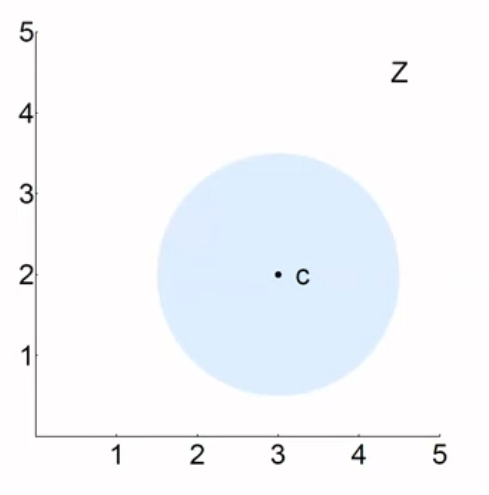
\includegraphics[width=0.6\textwidth, keepaspectratio]{./images/ball_arithm.png}
Также мы определяем все операции и тут происходит гораздо меньшая потеря точности, чем при представлении комплексных
интервальных чисел в виде пара вещественная и мнимая часть.
Интервальная арифметика не стала популярной. Наглядный пример
\[
\int_0^1 f(x)\,dx \approx \frac{1}{1000000} \sum_{k=1}^{1000000} f\left(\frac{k}{1000000}\right)
\]
Пусть f(s) вычисляется со случайной ошибкой порядка $\theta$.

Ожидаемая ошибка при вычислении суммы
\[
\sum_{k=1}^{1000000} f\left(\frac{k}{1000000}\right)
\]
будет порядка $\sqrt{1000000}\theta$ = 1000$\theta$.

\item[] Интервальная арифметика дает интервал с шириной порядка 1000000$\theta$.

\item[] Это возникает, потому что на каждом шаге сложения мы выбираем самый пессимистический случай, когда погрешности не сокращаются,
а всегда складываются.

\end{itemize} 

\section{Таблица}
\paragraph{}

\begin{tabular}{|c|c|c|c|}
    \hline
    \rule{0pt}{20pt}\shortstack{Числа в\\математике} & \shortstack{В аппаратуре\\(hardware)} & \shortstack{В языках\\программирования} & \shortstack{В символьных\\вычислениях} \\ \hline
    \rule{0pt}{20pt}Натуральные & 32bit, 64bit & диапазон 0..$2^{64}$ - 1 & \shortstack{зависит от кол-ва\\ оперативной памяти} \\ \hline
    \rule{0pt}{15pt}Ноль & +-0 & +-0 & \shortstack{зависит от \\организации кода} \\ \hline
    \rule{0pt}{20pt}Целые & 32bit, 64bit & диапазон $-2^{63}$..$2^{63}-1$ & \shortstack{зависит от кол-ва\\ оперативной памяти} \\ \hline
    \rule{0pt}{20pt}Рациональные & \shortstack{опирается на \\натуральные и целые} & \shortstack{существует тип \\данных Rational} & \shortstack{зависит от кол-ва\\ оперативной памяти} \\ \hline
    \rule{0pt}{20pt}Алгебраические & $\sqrt{x}$ & PARI, Calcium & \shortstack{зависит от кол-ва\\ оперативной памяти} \\ \hline
    \rule{0pt}{20pt}Вещественные & IEEE 754 & Интервалы &  \\ \hline
    \rule{0pt}{20pt}Комплексные & IEEE 754 & ComplexF64 &  \\ \hline
\end{tabular}

\end{document}
